\section{Auswertung}
\label{sec:Auswertung}


Die Graphen werden sowohl mit Matplotlib \cite{matplotlib} als auch NumPy \cite{numpy} erstellt. Die Fehlerrechnung wird mithilfe von Uncertainties \cite{uncertainties} durchgeführt. Mit der Tiefenmessung wird der Zylinder der Länge $l=\SI{120,5e-3}{\metre}$ vermessen. Mit der Schallgeschwindigkeit in Acryl von $c_.{Acryl}=\SI{2730}{\meter\per\second}$ \cite{cAcryl} ergibt sich für die Länge: $l_.{Tiefenmessung}=\SI{120.04e-3}{\metre}$.

\subsection{Bestimmung der Schallgeschwindigkeit mit Impuls-Echo-Verfahren}

\begin{table}
	\centering
	\caption{Die gemessenen Zeiten $t_1$ und $t_2$ am Anfang des Zylinders, sowie die Zeitdifferenzen $\Delta t_.{mess}$ und $\Delta t_.{eff}$ für die Acryl-Zylinder der Länge $l$ bei dem Impuls-Echo-Verfahren.}
	\label{tab:tabSchallgeschwindigkeit}
	\sisetup{table-format=1.2}
	\begin{tabular}{S[table-format=1.1]S[table-format=2.1]S[table-format=2.1]S[table-format=2.2]S[table-format=2.2]}
		\toprule
		{$t_.1/10^{-6}\si{\second}$} & {$t_.2/10^{-6}\si{\second}$} & {$\Delta t_.{mess}/10^{-6}\si{\second}$} & {$\Delta t_.{eff}/10^{-6}\si{\second}$} & {$l/10^{-2}\si{\metre}$} \\
		\midrule
		0.3 & 89.3 & 89.0 & 44.50 & 12.05 \\
		0.3 & 82.9 & 82.6 & 41.30 & 11.15 \\
		0.3 & 76.4 & 76.1 & 38.05 & 10.21 \\
		0.3 & 60.3 & 60.0 & 30.00 & 8.04 \\
		0.3 & 53.0 & 52.7 & 26.35 & 7.08 \\
		0.3 & 46.0 & 45.7 & 22.85 & 6.05 \\
		0.3 & 29.5 & 29.2 & 14.60 & 3.97 \\
		0.3 & 23.6 & 23.3 & 11.65 & 3.11 \\
		\bottomrule
	\end{tabular}

	\label{tab:SchallIE}
\end{table}

\noindent In der Abbildung \ref{fig:SchallIE} sind die Messwertepaare aus Tabelle \ref{tab:SchallIE} mit $\Delta t_.{eff}$ aufgetragen und durch einen linearen Fit der Form $l=c_1 t + l_{0,1}$ genähert:
\begin{align*}
	c_1&=\SI{2708(17)}{\meter\per\second}\text{,}\\
	l_{0,1}&=\SI{-6(5)e-4}{\meter}\text{.}
\end{align*}
Dabei ist $c$ die Schallgeschwindigkeit in Acryl und $l_0$ ist die Dicke der Anpassungsschicht. $\Delta t_.{eff}$ ist die Zeispanne, die der Schall für das einmalige Durchlaufen des Acrylzylinders benötigt. Sie beträgt dementsprechend die Hälfte von $\Delta t_.{mess}$, da der Acrylzylinder beim Impuls-Echo-Verfahren zwei mal vom Schall durchlaufen wird.

\begin{figure}
	\centering
	\caption{Die bei einer Laufzeit $t$ zurückgelegte Strecke $l$ des Schalls im Zylinder bei dem Impuls-Echo-Verfahren aufgetragen gegen die Laufzeit $t$.}
	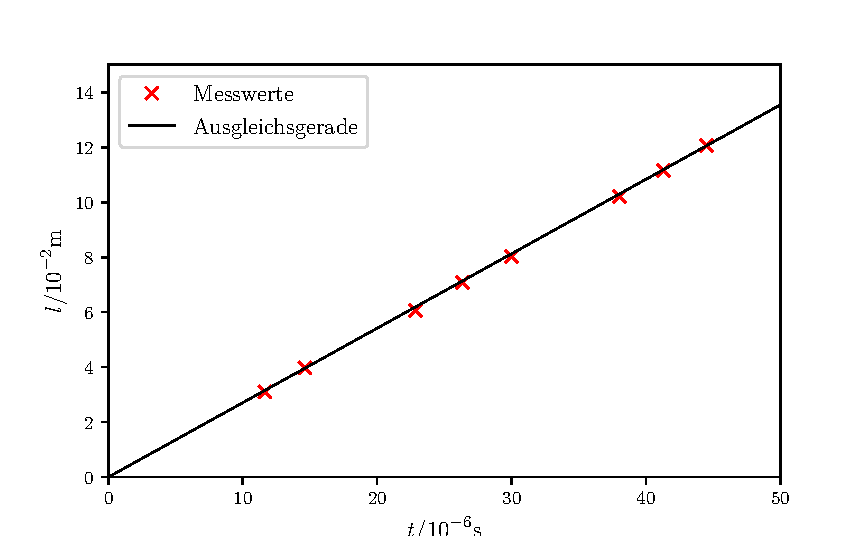
\includegraphics[width=\linewidth-70pt,height=\textheight-70pt,keepaspectratio]{content/images/Schallgeschwindigkeit.pdf}
	\label{fig:SchallIE}
\end{figure}

\subsection{Bestimmung der Schallgeschwindigkeit mit Durchschallungs-Verfahren}

\begin{table}
	\centering
	\caption{Die gemessenen Zeitdifferenzen $\Delta t_.{Durchschallung}$ für die Acryl-Zylinder der Länge $l$ bei dem Durchschallungs-Verfahren.}
	\label{tab:tabSchallgeschwindigkeitDurchschallung}
	\sisetup{table-format=1.2}
	\begin{tabular}{S[table-format=2.1]S[table-format=2.2]}
		\toprule
		{$\Delta t_.{Durchschallung}/\si{\second}$} & {$l/10^{-2}\si{\metre}$} \\
		\midrule
		44.5 & 12.05 \\
		41.3 & 11.15 \\
		38.0 & 10.21 \\
		30.0 & 8.04 \\
		26.4 & 7.08 \\
		22.9 & 6.05 \\
		14.6 & 3.97 \\
		11.7 & 3.11 \\
		\bottomrule
	\end{tabular}

	\label{tab:SchallD}
\end{table}

\noindent In der Abbildung \ref{fig:SchallD} sind die Messwertepaare aus Tabelle \ref{tab:SchallD} aufgetragen und durch einen linearen Fit der Form $l=c_2 t + l_{0,2}$ genähert:
\begin{align*}
	c_2&=\SI{2700(120)}{\meter\per\second}\text{,}\\
	l_{0,2}&=\SI{-4(4)e-3}{\meter}\text{.}
\end{align*}
Dabei ist $c$ die Schallgeschwindigkeit in Acryl und $l_0$ ist die Dicke der Anpassungsschicht.

\begin{figure}
	\centering
	\caption{Die bei einer Laufzeit $t$ zurückgelegte Strecke $l$ des Schalls im Zylinder bei dem Durchschallungs-Verfahren aufgetragen gegen die Laufzeit $t$.}
	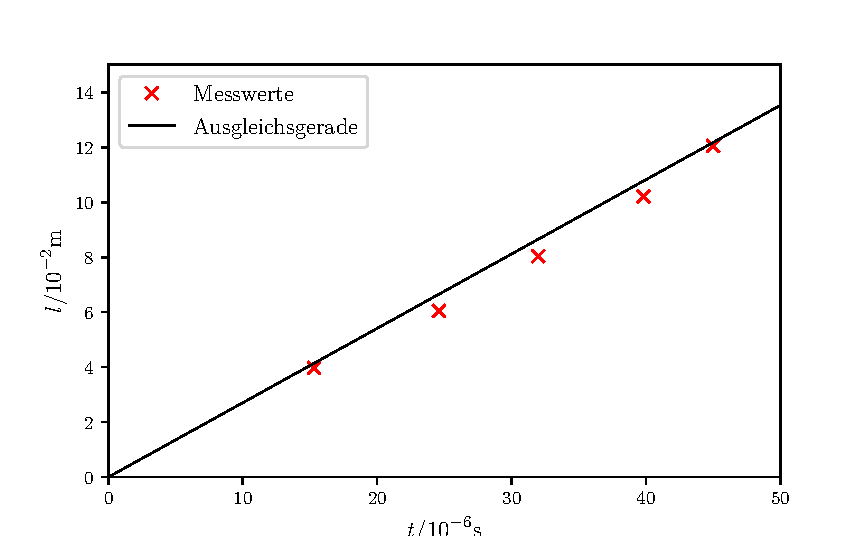
\includegraphics[width=\linewidth-70pt,height=\textheight-70pt,keepaspectratio]{content/images/SchallgeschwindigkeitDurchschallung.pdf}
	\label{fig:SchallD}
\end{figure}

\subsection{Bestimmung der Dämpfungskonstanten mit Impuls-Echo-Verfahren}

\begin{table}
	\centering
	\caption{Die gemessene Spannungsdifferenz $\Delta U$ zur ursprünglichen Spannung für die Acryl-Zylinder der Länge $l$ bei dem Impuls-Echo-Verfahren.}
	\label{tab:tabDaempfung}
	\sisetup{table-format=1.2}
	\begin{tabular}{S[table-format=2.2]S[table-format=1.3]}
		\toprule
		{$l/10^{-2}\si{\metre}$} & {$\Delta U/\si{\volt}$} \\
		\midrule
		12.05 & 1.391 \\
		10.21 & 1.336 \\
		8.06 & 0.312 \\
		8.04 & 0.363 \\
		6.05 & 0.156 \\
		3.97 & 0.131 \\
		3.11 & 0.095 \\
		\bottomrule
	\end{tabular}

	\label{tab:Daempfung}
\end{table}

\noindent In der Abbildung \ref{fig:Daempfung} ist der Logarithmus von der ursprünglichen Spannung $U$ gegen die zurückgelegte Strecke $l$ des Schalls im Zylinder mit den Werten aus Tabelle \ref{tab:Daempfung} aufgetragen und wird durch einen linearen Fit der Form $\ln(U)=-\frac{\alpha}{2} x + ln(U_0)$ genähert:
\begin{align*}
	\alpha	&= \SI{61(17)}{\per\meter}\text{,}\\
	ln(U_0)	&=\SI{1.8(7)}{}\text{.}
\end{align*}
Dabei ist $\alpha$ die Dämpfung. Die Ausgleichsformel ergibt sich aus Formel \eqref{eq:I}, unter berücksichtigung, dass $I\propto U^2$ gilt.
Aufgrund der schlechten Messwerte werden zwei weitere Näherungen derselben Form durchgeführt, einmal ohne die beiden letzten Werte (Interpretation1 in Abbildung \ref{fig:Daempfung}) und einmal ohne die vier mittleren Werte (Interpretation2 in Abbildung \ref{fig:Daempfung}). Diese liefern die Werte
\begin{align*}
	\alpha_{I1} &= \SI{8(2)}{\per\meter}\text{,}\\
	ln(U_{0,I1})&=\SI{0.47(5)}{}\text{,}
\end{align*} 
für die erste Interpretation und
\begin{align*}
	\alpha_{I2} &= \SI{61(2)}{\per\meter}\text{,}\\
	ln(U_{0,I2})&=\SI{1.3(1)}{}\text{,}
\end{align*}
für die zweite Interpretation.

\begin{figure}
	\centering
	\caption{Der Logarithmus von den beim Impuls-Echo-Verfahren bestimmten Spannungen $U$ aufgetragen gegen die im Zylinder nach der Zeit $t$ zurückgelegte Strecke $l$ des Schalls.}
	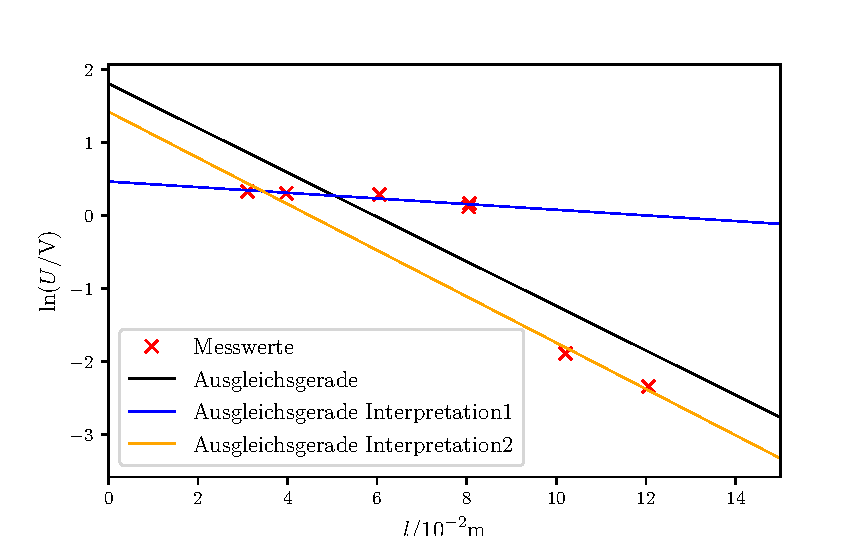
\includegraphics[width=\linewidth-70pt,height=\textheight-70pt,keepaspectratio]{content/images/Daempfung.pdf}
	\label{fig:Daempfung}
\end{figure}

\subsection{Untersuchung des Cepstrums/Spektrums}

\begin{table}
	\centering
	\caption{Die gemessene Länge/Dicke $d_.{mess}$ des Acrylzylinders und der Acrylplatten, sowie die gemessene Zeit im Spektrum bei dem Impuls-Echo-Verfahren.}
	\label{tab:tabMehrfachecho}
	\sisetup{table-format=1.2}
	\begin{tabular}{S[table-format=1.2]S[table-format=2.1]S[table-format=2.2]S[table-format=1.2]}
		\toprule
		{$d_.{mess}/10^{-2}\si{\metre}$} & {$\Delta t_.{mess}/10^{-6}\si{\second}$} & {$\Delta t_.{eff}/10^{-6}\si{\second}$} & {$d_.{exp}/10^{-2}\si{\metre}$} \\
		\midrule
		3.97 & 29.2 & 14.60 & 3.99 \\
		0.60 & 4.5 & 2.25 & 0.61 \\
		0.98 & 7.2 & 3.60 & 0.98 \\
		\bottomrule
	\end{tabular}

	\label{tab:Cepstrum}
\end{table}

\noindent Bei der Fourier transformierten ist ein Maximum bei $\SI{2.27}{\mega\hertz}$ zu erkennen.
Die Laufzeiten des Schalls in den Acrylplatten lassen sich aus dem Cepstrum zu $\Delta t_1=\SI{4.4e-6}{\second}$ und $\Delta t_2=\SI{7.2e-6}{\second}$ bestimmen. Die Laufzeit für beide Platten zusammen beträgt $\Delta t_{1+2}=\SI{11.6e-6}{\second}$. 
Mit der bekannten Schallgeschwindigkeit in Acryl von $c_.{Acryl}=\SI{2730}{\meter\per\second}$ \cite{cAcryl} ergeben sich somit für die Dicken der Platten:
\begin{align*}
D_{1,1}&=\SI{0.60e-2}{\meter}\text{,}\\
D_{1,2}&=\SI{0.98e-2}{\meter}\text{.}\\
\end{align*}
Mit den Werten aus Tabelle \ref{tab:Cepstrum} ergeben sich die Dicken der Platten bestimmt aus dem Spektrum:
\begin{align*}
D_{2,1}&=\SI{0.61e-2}{\meter}\text{,}\\
D_{2,2}&=\SI{0.98e-2}{\meter}\text{.}\\
\end{align*}

\begin{figure}
	\centering
	\caption{Die Messergebnisse für das Cepstrum.}
	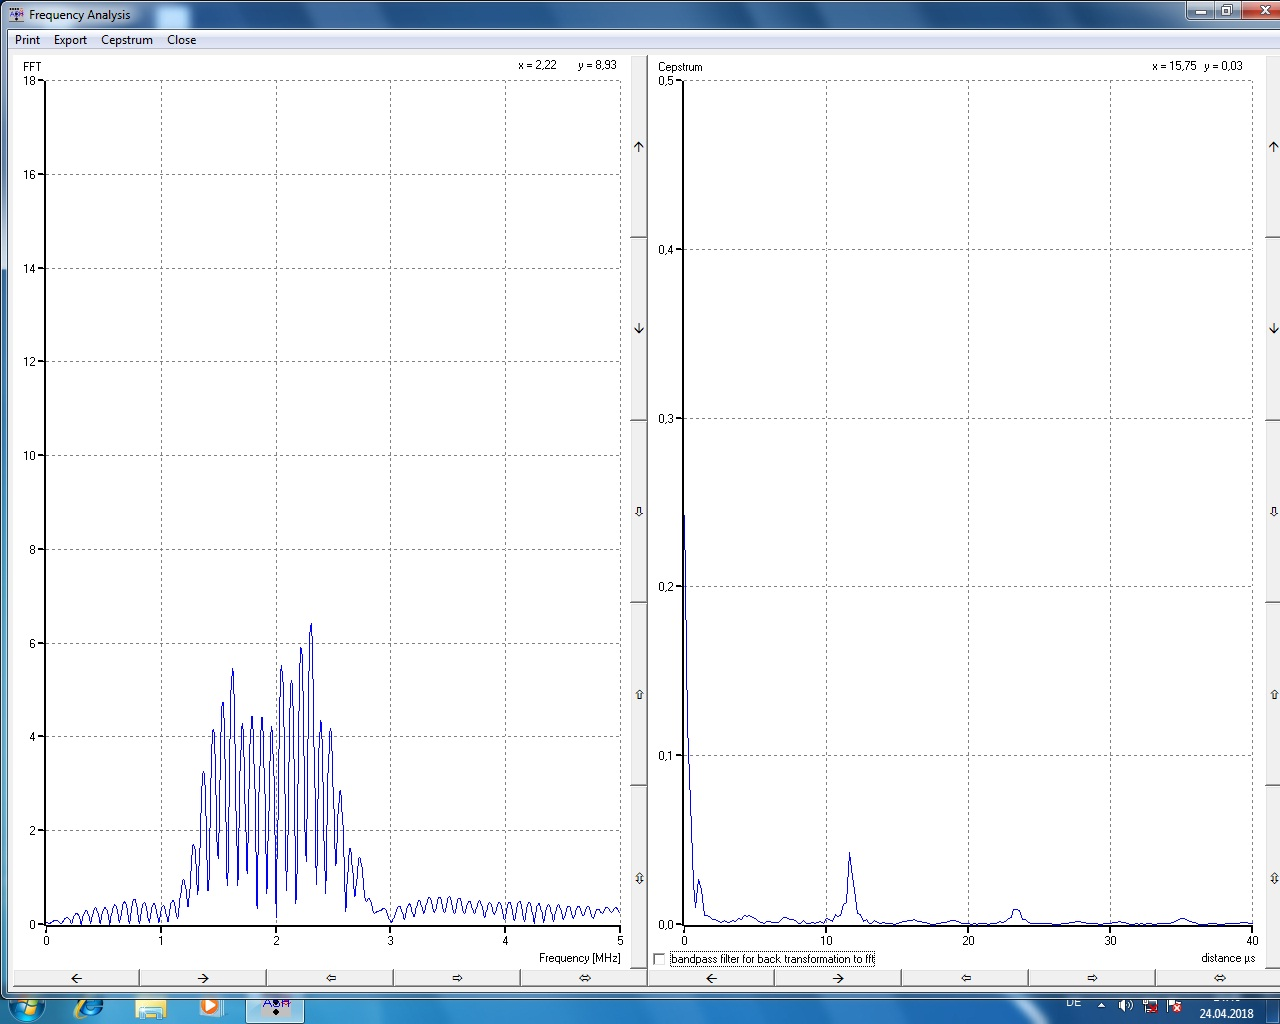
\includegraphics[width=\linewidth-30pt,height=\textheight-30pt,keepaspectratio]{content/images/CEPSTRUM.jpg}
	\label{fig:Cepstrum}
\end{figure}

\subsection{Untersuchung der Abstände in einem Augenmodell}

\noindent Mit den Werten für die Laufzeiten des Schalls im Auge aus Tabelle \ref{tab:Auge} lässt sich mit den bekannten Schallgeschwindigkeiten von $c_.{GK}=\SI{1410}{\meter\per\second}$ \cite{US1} außerhalb der Linse und von $c_.{L}=\SI{2500}{\meter\per\second}$ \cite{US1} in der Linse die Abstände im Augenmodell mit $s=vt$ berechnen. Dabei muss immer aufgrund der Impuls-Echo-Messung die jeweilige Zeitdifferenz durch zwei geteilt werden. Für den Abstand zwischen der Hornhaut und der Iris ergibt sich:
\begin{equation*}
A_1=\SI{7.33e-3}{\meter}\text{.}
\end{equation*}
Für den Abstand zwischen Iris und Linse ergibt sich:
\begin{equation*}
A_2=\SI{4.09e-3}{\meter}\text{.}
\end{equation*}
Für die Dicke der Linse ergibt sich:
\begin{equation*}
A_3=\SI{8.90e-3}{\meter}\text{.}
\end{equation*}
Für den Abstand zwischen Linse und Retina ergibt sich:
\begin{equation*}
A_4=\SI{35,3e-3}{\meter}\text{.}
\end{equation*}
Bei dem vierten Wert handelt es sich wahrscheinlich um eine Doppelreflexion an der Linse.
Das Spektrum der Messung ist in Abbildung \ref{fig:Auge} zu sehen.

\begin{table}
	\centering
	\caption{Die Werte für die Laufzeiten $\Delta t_A$ des Schalls für die Abstände im Augenmodell.}
	\label{tab:tabAuge}
	\sisetup{table-format=1.2}
	\begin{tabular}{S[table-format=1.0]S[table-format=2.1]}
		\toprule
		{$n$} & {$\Delta t_.A/10^{-6}\si{\second}$} \\
		\midrule
		1 & 10.4 \\
		2 & 16.2 \\
		3 & 23.3 \\
		4 & 31.6 \\
		5 & 73.4 \\
		\bottomrule
	\end{tabular}

	\label{tab:Auge}
\end{table}

\begin{figure}
	\centering
	\caption{Die Messergebnisse für das Augenmodell.}
	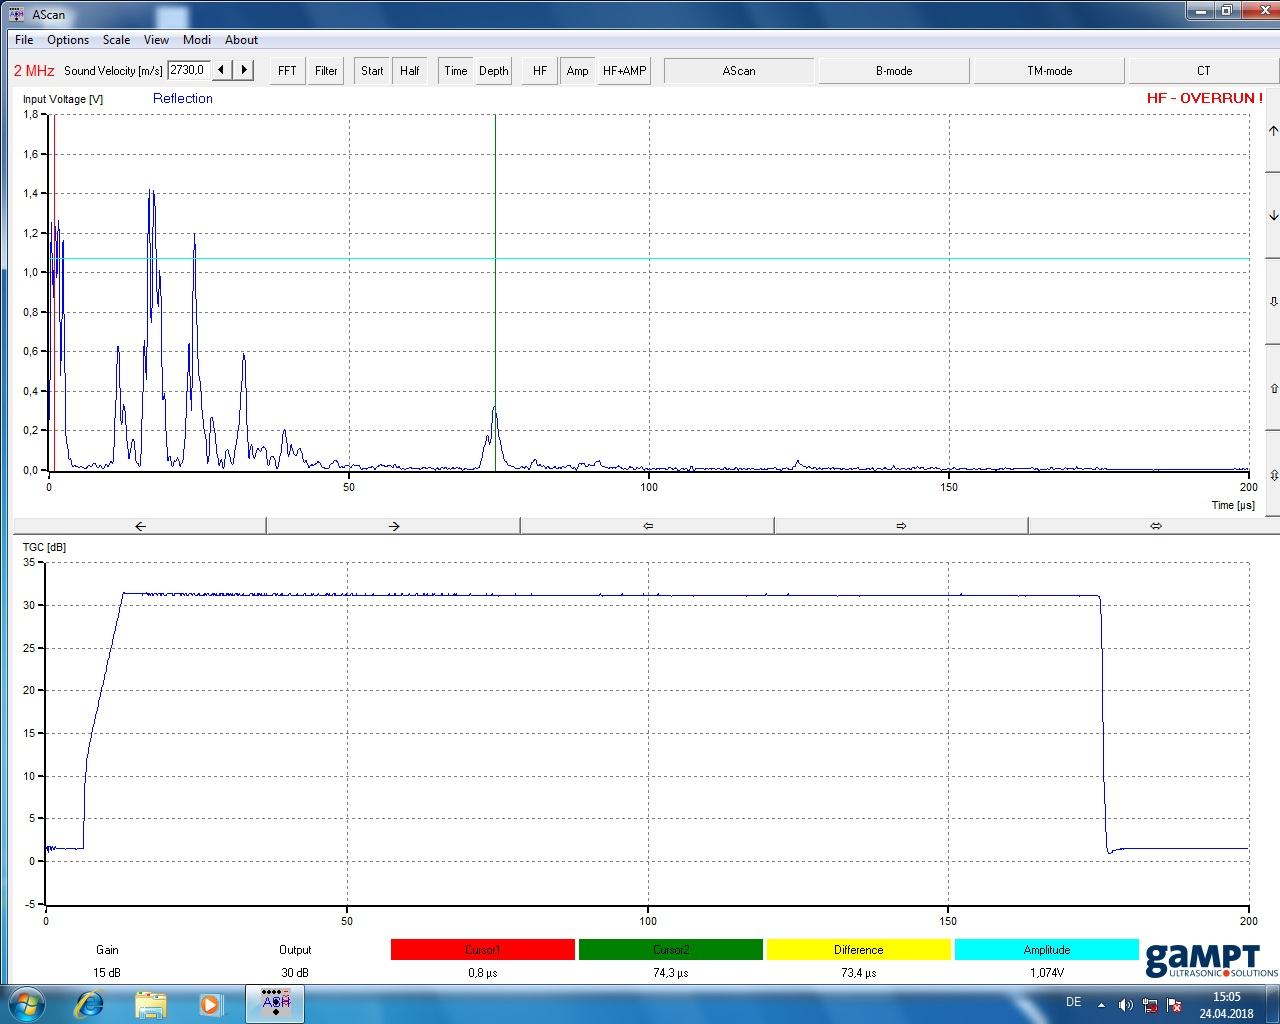
\includegraphics[width=\linewidth-30pt,height=\textheight-30pt,keepaspectratio]{content/images/AUGE.jpg}
	\label{fig:Auge}
\end{figure}